%% LaTeX2e class for student theses
%% sections/content.tex
%% 
%% Karlsruhe Institute of Technology
%% Institute for Program Structures and Data Organization
%% Chair for Software Design and Quality (SDQ)
%%
%% Dr.-Ing. Erik Burger
%% burger@kit.edu
%%
%% Version 1.3.2, 2017-08-01
\chapter{Abstract}
The amount of data created by high energy experiments will drastically increase in the next years and cannot be processed without an efficiently resource usage.
To achieve a better resource utilization the load balancing strategies have to be optimized.
However, such optimization are tedious and error prone for large and complex computing systems without the help of simulations.

To improve the load balancing of the World Wide LHC Computing Grid (WLCG) we model and simulate the performance of computing jobs executed at the Tier 1 centre GridKa.
This model is validated using real world data and enables us to evaluate various load balancing strategies.


\chapter{Motivation}
The WLCG is one of the largest grids in the world and processes the data created by the Large Hadron Collider (LHC) at CERN \cite{wlcg_update}. 
The amount of data to be processed steadily increases, expecting about 50 Petabytes in 2018. Therefore, the grid has to be constantly extended and optimized to be able to handle the increasing load.

Nevertheless, the amount of data will drastically increase in the coming years due the upgrade of the LHC to the High-Luminosity Large Hadron Collider (HL-LHC), creating major challenges for the community of HEP \cite{community}.
The goals of the HL-LHC upgrade include the search for dark matter, the investigation of matter-antimatter differences and exploiting the discovery of the Higgs boson as a precision tool.
\Cref{resources} shows the estimated CPU resources for the ATLAS experiment in the next ten years. As can be seen there is a large gap between needed resources and estimated resources in 2026 till 2028. This gap is created due the start of the HL-LHC era, which requires much more computing resources. One approach to close this gap is to improve the load balancing strategy. 

\begin{figure}
	\centering
	\includegraphics[width=1.0\linewidth]{images/resources}
	\caption[]{Estimated CPU resources of ATLAS \cite{community}}
	\label{resources}
\end{figure}



However, there is currently no model or simulation existing to evaluate the load balancing strategies of the grid, helping the operators to make the correct decisions in the optimization process.
Optimizing load strategies without the help of simulations requires stable load, in order to preserve the comparability of the different strategies. This is neither possible to achieve for the WLCG nor for a single centre like GridKa, because the nature of the load is highly dynamically. Another option would be to use an isolated test system for the evaluation. However, the system under inspection is too large and thus a similar test systems would not be financially affordable. A smaller test system could not deliver correct results because too much of the complexity would be taken away.
These reasons lead to the conclusion that a model and simulation of the performance of computing jobs is required to evaluate different load balancing strategies.

Our long term goal is to evaluate different load balancing strategies for the WLCG and additionally evaluate different design decisions affecting the performance of the grid. These gained insights will help the HEP community to solve the challenges created by the HL-LHC upgrade.
The first step to archive this goal is to model and simulate the performance of computing jobs at the Tier 1 centre GridKa.
The model and simulation will be created using Palladio, which leads to the research question which extensions to Palladio are required to achieve accurate results that can be used to evaluate load balancing strategies for GridKa.

This model enables us to evaluate strategies for GridKa and allows us to draw conclusions about the best optimizations of the load balancing for the WLCG. Furthermore, it can be used as a foundation for models and simulations of larger parts of the WLCG.


The following sections describe the WLCG in detail, the current state of the load balancing, and the desired state in the future.

\section{Worldwide LHC Computing Grid}

The WLCG processes 50 Petabytes of data each year created by the LHC at CERN \cite{data_process}
and with its help the Higgs boson was discovered in 2012 \cite{wlcg_online}.

Over 170 computing centres distributed over 42 countries are part of the WLCG and it combines over 72.000 CPUs, 386 Petabytes online data space and 368 Petabytes nearline space (tape storage) \cite{wlcg_data}. Every day it runs about 2 million jobs to analyse data of the CERN experiments.

At CERN there are four experiments taking place, namely: Atlas, Alice, CMS, and LHCb. They all use the grid in a similar, but not the same way \cite{wlcg_computing}. \Cref{fig:wlcg} shows the hierarchical three tier structure of the WLCG. Tier 0 is the CERN compute centre, which stores all raw data of the experiments, makes the first pass reconstruction and distributes raw data to Tier 1 compute centres. Tier 1 consists of 13 sites, which store a share of raw and reconstructed data, creating a second copy. They also run analysis and simulation jobs. Tier 2 sites, which are mostly located at universities or other scientific institutes, do monte carlo production. In contrast to Tier 1 sites, the Tier 2 sites do not have much storage \cite{wlcg_computing}.

The WLCG is heterogeneous, meaning that the resources of one site are different to the resources of another site, the network connections between sites vary, and even the nodes in a single site have different resources. It is trending to use more virtualization, resulting in even more heterogeneity \cite{wlcg_update}.

Our work will focus on modelling and simulating load balancing strategies for the CMS experiment. Yet the results of our work can be presumably transferred to the other experiments, because they all use the grid in a similar way.

	\begin{figure}[t!]
		\centering
		\includegraphics[width=0.9\linewidth]{images/WLCG}
		\caption[]{Tier structure of the WLCG \cite{wlcg_tiers}}
		\label{fig:wlcg}
	\end{figure}
	

\section{Current State}
Currently, the load balancing strategy used at the CMS computing model is improvable.
One aspect is that it does not account the nature of the jobs: simulation jobs require heavy I/O load and analysis jobs require heavy CPU time \cite{1742-6596-331-7-072038}. If this nature is not accounted in the scheduling decision, it leads to a bad utilization of the nodes. A good strategy would schedule the right amount of simulation and analysis jobs to a site to maximize the utilization of I/O and CPU. For example, if too many simulation jobs are scheduled, the I/O is creating a bottleneck and the CPUs are idling. There are several other ideas how the load balancing could be improved, but they cannot be evaluated without a simulation.

Another approach to improve the CMS computing model is to upgrade the grid infrastructure such as integration of cloud computing resources or creation of better links between the sites. A simulation could help to find the best improvement in terms of speed-up, cost or utilization.


\section{Envisioned Solution} 
The amount of data produced by the LHC is steadily increasing, thus either more computing resources have to be provided or the existing ones have to be used in a more efficient way.
However, the computing resources will not increase in the same magnitude as the produced data, hence a better utilization of the given resources is required. Our approach will allow to simulate the effects of different load balancing strategies and decide on these results what the best strategy is. The scheduling problem itself is np complete, so the optimal solution will not be found, but we can decide on a set of strategies which one is the best \cite{1698650}. Evaluating load balancing strategies using the productive system is not accurate, because the workload constantly changes. This makes the performance results of different load balancing strategies incomparable. Though, this problem will be solved by using simulations.

Furthermore, our approach can be used to evaluate the effects of changing the infrastructure of the grid. Therefore, we can find the best approach to improve the CMS computing model, e.g. adding cache, create a new network connection or allow dynamic appearing nodes.
It is difficult to find the best approach without using a simulation, because one cannot consider all side-effects of a change. For example increasing the CPU resources may be a bad decision, because then the network would become the bottleneck. Only the increasing of both, the network and the CPU resources, would lead to an improvement.


\chapter {State of the Art}
In this chapter four simulators are presented which could be used to model and simulate GridKa, from which we chose Palladio to use in this project. There are several other simulators existing, but these are the most relevant ones.

It should be noted that there is no indication that a similar large system like GridKa has been simulated before. Our work will figure out if it is possible to model and simulate such large systems with the current state of simulators.

\section{Palladio}
\label{palladio}
Palladio is a model driven software architecture simulator developed by Karlsruhe Institute of Technology (KIT), FZI Research Center for Information Technology, and University of Paderborn. The development started in 2003 and it is still actively developed today. Palladio predicts quality of software properties (e.g. performance) using several models of a system \cite{BECKER20093}.

These models are the component model, the assembly model, the resource model, the allocation model, and the usage model.
The component model specifies the structure and behaviour of the components independently from their later usage. This allows reuse of the components, but requires its parametrization.
To represent how the components are connected to model the software architecture, the assembly model has to be created. 
The resource model describes the resource environment. It contains the number and characteristics of the resource containers on which the components could be deployed and the topology of the network connecting these containers.
Allocation models represent the mapping of the different components to the resource containers.
Finally, the usage model defines how a system is used regarding workload, user behaviour, and parameters.

Once these models are created, Palladio can be used to simulate the system choosing one of several supported simulators. \Cref{fig:palladio} shows the modelling and simulation process. 

Lehrig and Becker \cite{arch} extended Palladio with Architectural Templates to make it possible to model cloud computing environments efficiently.

Furthermore, Palladio's simulation approach SimuLizar was created to simulate self-adaptive systems \cite{becker2013simulizar}.
It was later extended to support the metrics scalability, elasticity, and efficiency \cite{arch}.

The first case studies using Palladio in cloud environments show that it delivers accurate results \cite{arch}. However, Palladio was never used to model and simulate such a large system as the CMS computing model.

\begin{figure}
	\centering
	\includegraphics[width=1\linewidth]{images/palladio}
	\caption[]{Process of Palladio \cite{BECKER20093}}
	\label{fig:palladio}
\end{figure}


\section{MONARC}
The MONARC project was started 1998 to help develop the initial design of the WLCG at CERN \cite{monarc2000models}.
To simulate possible structures of the WLCG they created the MONARC simulator.
The results of the simulations indicated that a hierarchical structure with regional centres performs best, resulting in the three Tier structure of the WLCG today \cite{morita2001validation}. 
After its initial results, the MONARC project proposed to model, prototype, and optimise the design of the overall distributed computing and data handling systems for the LHC experiments \cite{monarc2000models}.
However, the project was not continued in 2000.

2004 a second version of the MONARC simulator was released with several improvements, such as simulation of data replication. MONARC2 focuses on simulating experiments at CERN, but can also be used to simulate general large scale distributed computing systems \cite{legrand2003monarc}. A major difference to its first version is, that a discrete-event approach instead of a discrete time-stepped is used, which results in a better performance.

2010 Zach et al. \cite{1742-6596-331-7-072038} used MONARC2 to simulate the ALICE Tier-2 site in Prague. The simulation included 3000 CPUs, and the CPU as well as the network and I/O resources were simulated. MONARC2 delivered accurate simulation results, however two problems occurred. Firstly they were not able to simulate the network load correctly and secondly MONARC2 revealed performance issues, making it not usable for even larger systems.
\newpage
\section{CACTOS}
CACTOS is an approach to cloud infrastructure automation and optimization, started in 2014 as a project funded by the European Union \cite{cactos}.
One part of the approach is the CACTOS Runtime Toolkit for monitoring and resource management and another part is the CACTOS Prediction Toolkit for evaluation of alternative data centre deployment scenarios and resource management algorithms.

The Prediction Toolkit is built on Palladio and SimuLizar, see \cref{palladio} for details on Palladio.
The models used by the Prediction Toolkit regarding resource or application behaviour are updated using monitoring data to handle the highly dynamic behaviour of clouds.
The idea to couple monitoring and grid simulation tools has been around for a while, suggested by Pop et al. \cite{1698650} in 2006.

CACTOS supports the rapid testing of resource management algorithms due the ability to simulate them without the need to reimplement the algorithms against the Prediction Toolkit. Most other simulators require the reimplementation of a resource management algorithm to its specific interface. Furthermore, it allows the automatic creation of workload models using runtime monitoring data \cite{rapidtesting}.

First case studies show that the Prediction Toolkit has a high accuracy, but it was not tested on large systems yet \cite{rapidtesting}. Nevertheless, CACTOS aim is to simulate cloud infrastructures, which leads to many features that are not needed to simulate GridKa. This feature richness would lead to big overhead when implementing load balancing strategies and worse performance regarding simulation time. Thus, CACTOS is not the best choice to model and simulate GridKa.


\section{SimGrid}
SimGrid is a framework for simulating large-scale distributed systems and one of the earliest created grid simulators \cite{simgrid_update}. Its first release was 1998 and is one of the few that is still developed today. Originally, it started as a grid simulator, but it became more versatile. Therefore it can be used as a grid, P2P, MPI, or cloud simulator today. Moreover, it is one of the most used grid simulators \cite{simgrid_update}.

In SimGrid the platforms and the deployment are defined in XML, and the application behaviour and scheduling is implemented using C. It supports simulation of CPU, I/O and network resources, heterogeneous workloads, and heterogeneous platforms \cite{simgrid_update}.

It is more scalable than GridSim, which is another popular grid simulator \cite{simgrid_update}.
This performance difference is created by several optimizations, including implementing light-weight execution contexts, using lazy activity updates, and using trace integration for resource management \cite{simgrid_update}.

However, without the help of graphical model editors the models of the computing jobs are time-consuming to create. The support of graphical editors is a big advantage of Palladio. 


\chapter{Exploratory Work}
We chose Palladio as the tool to model and simulate the performance of computing jobs executed at the Tier 1 centre GridKa. Therefore, the first step was to learn how to work with Palladio and explore its possibilities. Due this process the initial prototype of the model was created and the required improvements of Palladio were found. This initial model will be refined during the project and the different planned improvements are described in \cref{plan}.

Furthermore, we gathered performance data about the computing jobs and the resource environment at GridKa.
First of all, these data was analysed to assess its usefulness and verify that they contain all required information. The analysis showed that all required information about the resource environment is available (CPU, I/O and network performance). In addition, the computing job data contain nearly all required information (CPU usage, job type, job start time and job run time), unfortunately the I/O usage is missing.
Because the data contain nearly all required information we were able to calibrate the model and are working on receiving the I/O usage of the jobs, making the calibration more accurately.

One key question is if Palladio and SimuLizar are scalable enough to simulate such large systems in a satisfying time. \Cref{scal} shows the required simulation time for the initial model. It can be seen that even for long simulated times the required real time is acceptable.
These results suggest that Palladio will be scalable enough to simulate GridKa and even bigger parts of the WLCG, thus we will continue to use Palladio as the tool to model and simulate the computing jobs at GridKa. 

\begin{figure}[h]
	\begin{center}
		\caption{Simulation Times of Palladio}
		\label{scal}
		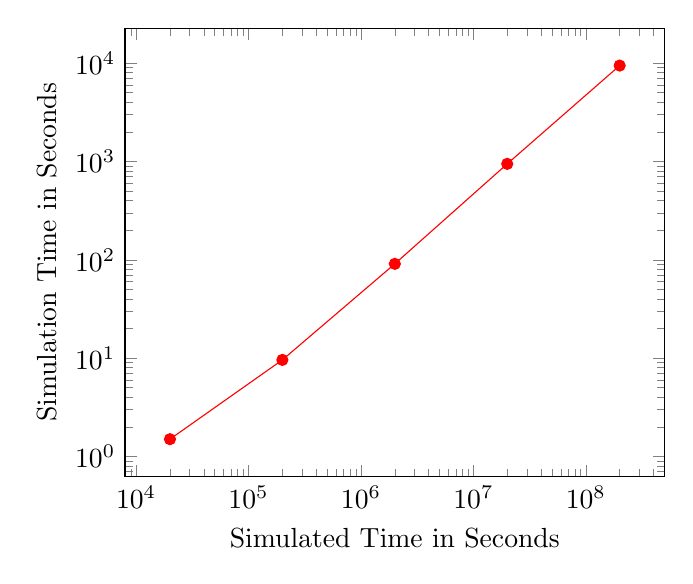
\begin{tikzpicture}
		\begin{loglogaxis}[
		xlabel={Simulated Time in Seconds},
		ylabel={Simulation Time in Seconds},
		]
		\addplot[color=red, mark=*] coordinates {
			(20000, 1.50)			
			(200000, 9.60)
	       	(2000000, 91.00)
			(20000000, 946.00)
		    (200000000, 9447.00)
	 };
		\end{loglogaxis}
		\end{tikzpicture}
	\end{center}
\end{figure}


\chapter{Goals and Methodology}
The goal of our work is to model and simulate the performance of computing jobs executed at the Tier 1 centre GridKa for the CMS computing model. The simulation should be accurate enough to allow the evaluation of different load balancing strategies and design decisions. Finally, the model will be validated using real world performance data. 

While creating the initial model several short comings of Palladio have been detected, which must be remedied to create accurate simulation results. 

This leads to the following sub goals that are described in detail in \cref{plan}: 
\begin{itemize}
	\item Model resource environment fine granularly: Currently it is not possible to model multiple types of resource containers. This is not accurately enough, instead each type of resource container at GridKa should have an own representation in the model.
	\item Generate measurement points: For each resource container the measurement points to measure the resource usage should be generated. It is not practical to create these measurement points manually for about 1000 resource containers.
	\item Model job slot concept: Each resource container can only run a certain amount of computing jobs in parallel, this is the amount of job slots a resource container has. We need to model this concept, because it is a foundation of the load balancing algorithm.
	\item Implement more realistically load balancing: Currently the load balancing algorithm randomly chooses the resource container. This does not reflect a realistically load balancing algorithm, therefore a load balancing algorithm based on available job slots should be implemented.
	\item Enable replay of traces: To be able to simulate and replay real world situations, Palladio should be able to replay traces of computing jobs at GridKa. This feature enables us to make the validation more accurately.
	\item Implement optional improvements: This sub goal contains several ideas how the model could be improved. In contrast to the other sub goals these improvements are optional because their effects are expected to be not as big as the effects of the other sub goals. 
	\item Validate model: The last goal is to validate the model. The validation consists of two part. In the first part the model is validated using real world data. In the second part a change of the load balancing strategy will be evaluated.
\end{itemize}


\chapter{Work Plan}
\label{plan}
Starting from the created initial model of the computing jobs at GridKa, Palladio and the model are improved.
The initial model describes the CPU usage and the arrival frequency of the computing jobs. In addition, it also models the resource containers on a coarse-grained level.

This project is carried out in collaboration with Maximilian Stemmer-Grabow's bachelor's thesis \textit{Calibrating Performance Models for Particle Physics Workloads}. In his bachelor's thesis, Stemmer-Grabow focuses on data extraction and model calibration, whereas this project focuses on remedying the short comings of Palladio.

In the following sections the different subtasks of this project are described. The time plan of the project is depicted in \cref{timeplan}.

\vspace*{\fill}
\begin{figure}[h]
	
\centering

\begin{ganttchart}[%Specs
x unit = 0.5cm,  %<---------------------- New x unit 
y unit title=0.5cm,
y unit chart=0.5cm,
vgrid, hgrid,
title height=1,
title label font=\bfseries\footnotesize,
bar/.style={fill=lightgray},
bar height=0.5,
group right shift=0,
group top shift=0.7,
group height=.3,
group peaks width={0.2},
inline]{1}{22}
%labels

\gantttitle[]{2018}{22} \\                 % title 
\gantttitle{Apr}{4}
\gantttitle{May}{5}
\gantttitle{Jun}{4}
\gantttitle{Jul}{5}
\gantttitle{Aug}{4}\\


% Setting group if any

\ganttgroup[inline=false]{Implementation}{2}{13} \\

\ganttbar[inline=false]{Fine granular Resources}{2}{2}\\
\ganttbar[inline=false]{Measurement Points}{3}{4} \\
\ganttbar[inline=false]{Job Slot Concept}{5}{6} \\
\ganttbar[inline=false]{Accurate Load Balancing}{7}{9} \\
\ganttbar[inline=false]{Replay}{10}{11} \\
\ganttbar[inline=false]{Optional Improvements}{12}{13} \\

\ganttgroup[inline=false]{Validation}{14}{16} \\
\ganttbar[inline=false]{Validation Part I}{14}{14} \\
\ganttbar[inline=false]{Validation Part II}{15}{16} \\



\ganttgroup[inline=false]{Paper}{14}{20} \\
\ganttbar[inline=false]{Writing Paper}{14}{20} \\
\ganttmilestone[inline=false]{Submit Paper}{20} \\ 

\end{ganttchart}
\caption[]{Time Plan}
\label{timeplan}
\end{figure}
\vspace*{\fill}
\clearpage
\section{Fine granular Resource Environment}
To represent the resource environment more fine granularly, the applied Architectural Template hast to be modified.
This template is applied to a resource container and specifies how many instances of this resource container should be generated in the completion phase.
Currently the template can only be applied to one resource container, hence we can only model on type of resource containers. Our approach is to extend the template so it can be applied to multiple types of resource containers.

The result of this subtask is that each type of resource container at GridKa can be modelled as a resource container in Palladio and that the Architectural Template can be applied to each of these resource containers, resulting in a more accurate simulation.
The expected effort for this subtask is about one week.

\section{Measurement Points Generation}
Measurement points are needed to evaluate the resource usage of each resource container. To create them automatically the Architectural Template plugin should be extended. The developer specifies the measurement points for each resource container, with the result that the measurement points for the generated resource containers should be created due the completion phase.

Without this feature the validation cannot take place, because it is not practical to manually create the measurement points for about 1000 resource containers. This feature requires about two weeks of work.

\section{Job Slot Concept}
In the CMS computing model one resource container can only run a limited amount of computing jobs in parallel. This is called the amount of job slots of a resource container. The job slot concept is a foundation for the load balancing strategy, because the load balancing looks for available job slots to deploy the computing job. To realize this concept, a new Architectural Template has to be created that wraps an allocation context. When applying the template the amount of job slots is specified. Architectural Templates then generate a component that acquires a job slot before the wrapped component is executed and releases it after the execution is finished.

After modelling the job slots, a more realistic load balancing strategy can be implemented. It is expected to take two weeks to implement the job slot concept. 
\clearpage
\section{Accurate Load Balancing}
\label{scheduling}
The decision on which resource container a computing job runs highly affects the quality of the simulation. In the initial model the jobs are randomly deployed. This behaviour is not close to reality, instead a load balancing strategy should be implement which considers the available job slots of a resource container. 

This requires the implementation of a new Palladio plugin that realizes the load balancing mechanism and its configurable strategies.
It is expected that this subtask requires the most work with about 3 weeks.

\section{Replay}
The ability to replay traces of computing jobs is valuable because it enables one to replay concrete time-spans and situations. Furthermore, this makes the validation more accurate. To simulate the used resources of the resource containers, the input trace file contains the job type, the arrival time, and the required resources of a job.

To implement the replay feature the plugin mentioned in \cref{scheduling} should be extended. The amount of work is estimated to be about two weeks.

\section{Optional Improvements}
This subtask contains several optional improvements which are expected to have not such a big impact on the quality of the model as the other subtasks, and thus are not as critical. This improvements includes the modelling of resource usage of other experiments at GridKa, data transfer from and to GridKa, modelling of individual phases of each job and modelling of pilot jobs.
This list of optional improvements is not complete and could be extended due the project.

The method to approach this subtask is depicted in \cref{iterative}. After implementing all other subtasks the model is compared with measured performance data. Based on these results the most promising improvement should be implemented. It is a iterative process, so after implementing one improvement the model is again compared with measured data to decide with which feature to continue.

The estimated time for this subtask is two weeks, however it will only be realised if there is enough time left, otherwise the time is used as a buffer.

\begin{figure}[h]
	\centering
	\includegraphics[width=1.0\linewidth]{images/method}
	\caption[]{Scientific method: theory-driven empiricism \cite{theory}}
	\label{iterative}
\end{figure}


\section{Validation}

The last subtask is the validation of the model to assess its quality. The validation consists of two parts; in the first part the model is compared with real world performance data to determine the differences of response times and resource usage.
Thereby, it is determined, how well the model reflects the performance of the computing jobs and the current load balancing.

In the second part the load balancing strategy is changed and this new load balancing strategy is evaluated.
The first part is expected to take one week and the second to take two weeks.
